\chapter{Bayesian Neural Networks}
% Authors: Jong Yeob Kim, Zilin Bian, Di Sha, 4/23/19.

In this section, we perform experiments using Bayesian neural networks. We show that Bayesian neural networks capture model uncertainty, which cannot be captured by standard neural networks or deep learning tools. 

\section{Libraries}

\begin{minted}{python}
import torch
from torch import nn, optim
from matplotlib import pyplot as plt
from plot_lib import set_default
\end{minted}

\section{Creating the data}
\begin{minted}{python}
# Set style (needs to be in a new cell)
set_default(figsize=(16, 8))

# Training set
m = 20  # nb of training pairs
x = (torch.rand(m) - 0.5) * 10  # inputs, sampled from -5 to +5
y = x * torch.sin(x)  # targets

# View training points
plt.plot(x.numpy(), y.numpy(), 'o')
plt.axis('equal')
plt.ylim([-10, 5])
\end{minted}

\begin{figure}[H]
    \centering
    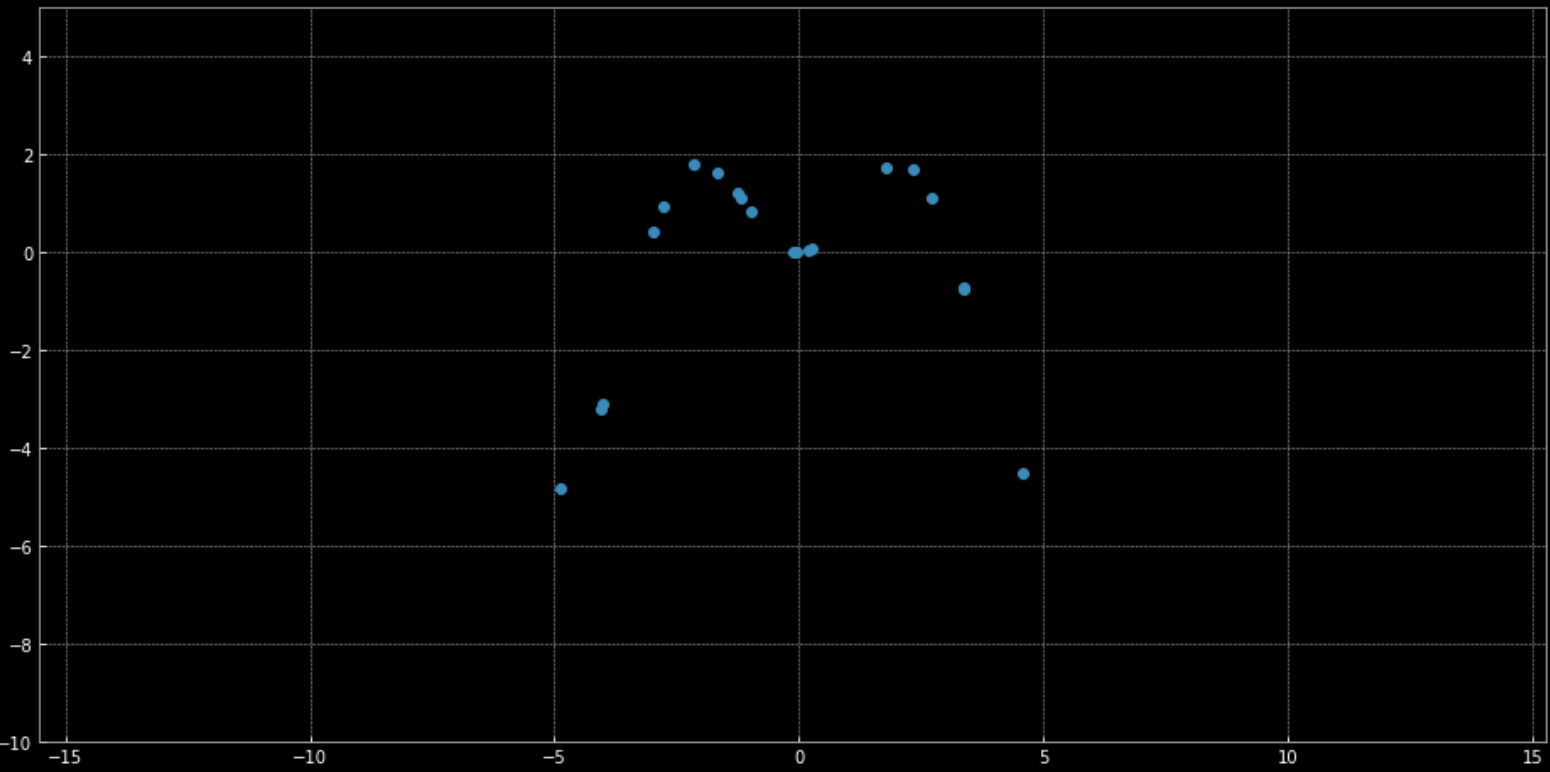
\includegraphics[width=\textwidth]{figs/exp_1.png}
    \caption{View training data}
    \label{fig:training_data}
\end{figure}

We define 20 training data points from -5 to +5. Now, we are going to fit a network over the data points.

\section{Experiments using Bayesian neural networks}
\begin{minted}{python}
# Define network architecture (try different non-linearities)

non_linear = nn.Tanh
# non_linear = nn.ReLU

net = nn.Sequential(
    nn.Dropout(p=0.05),
    nn.Linear(1, 20),
    non_linear(),
    nn.Dropout(p=0.05),
    nn.Linear(20, 20),
    non_linear(),
    nn.Linear(20, 1)
)
\end{minted}
In this neural network, the dropout acts directly on our inputs. We use tanh function for non-linearity in our first experiment.  

\begin{minted}{python}
# Training objective and optimiser
criterion = nn.MSELoss()
optimiser = optim.SGD(net.parameters(), lr=0.01, weight_decay=0.00001)

# Training loop
for epoch in range(1000):
    y_hat = net(x.view(-1, 1))
    loss = criterion(y_hat, y.view(-1, 1))
    optimiser.zero_grad()
    loss.backward()
    optimiser.step()
#     print(loss.item())

# Define a denser input range
xx = torch.linspace(-15, 15, 1000)

# Evaluate net over denser input (try both eval() and train() modes)

net.eval()
# net.train()

with torch.no_grad():
    plt.plot(xx.numpy(), net(xx.view(-1, 1)).squeeze().numpy(), 'C1')
plt.plot(x.numpy(), y.numpy(), 'oC0')
plt.axis('equal')
plt.ylim([-10, 5])
\end{minted}

\begin{figure}[H]
    \centering
    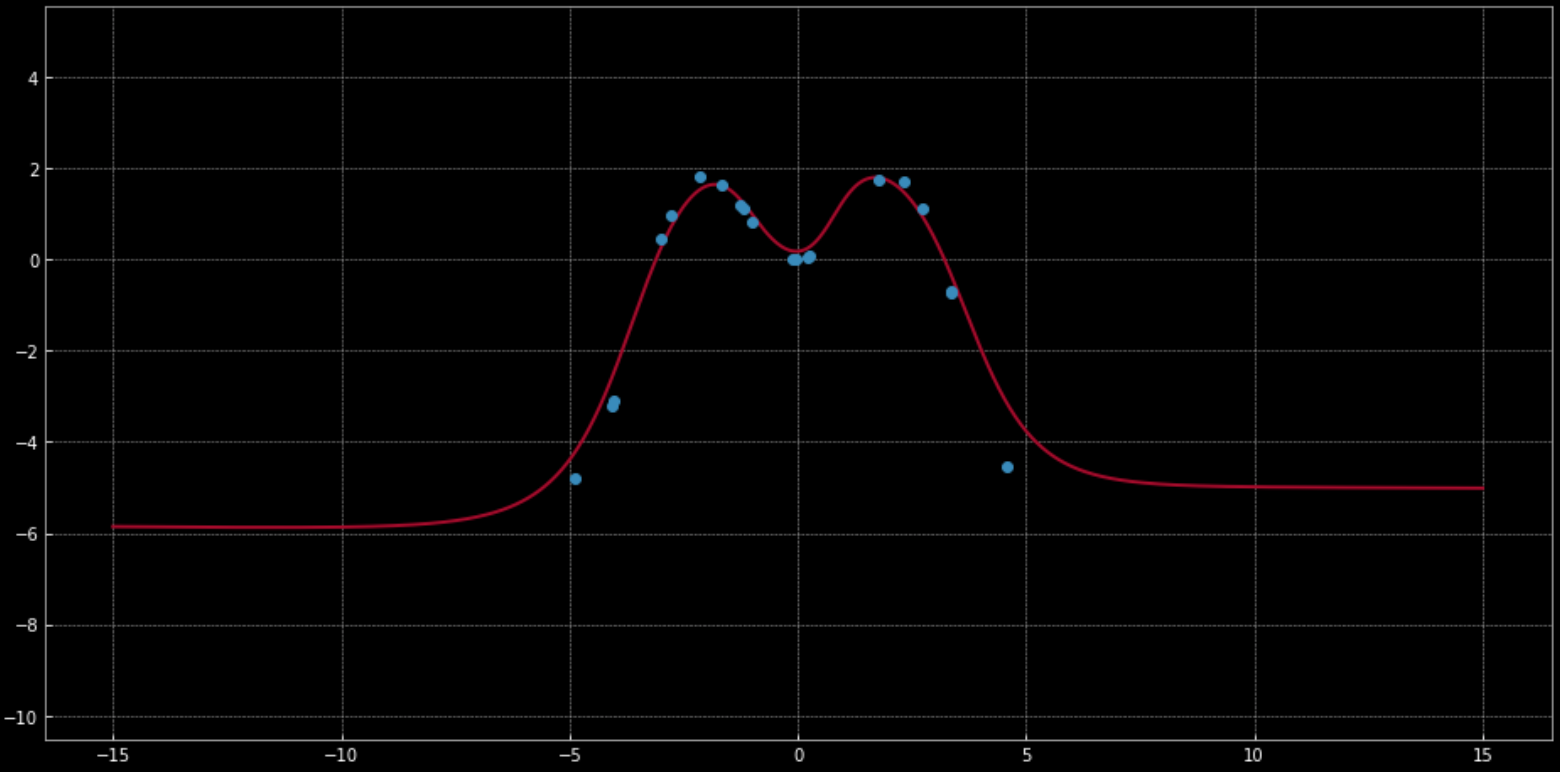
\includegraphics[width=\textwidth]{figs/exp_2.png}
    \caption{Fit standard neural network (with Tanh non-linearity)}
    \label{fig:fit_standardNN}
\end{figure}

We set to evaluation mode to turn-off the dropout. As we can see in Fig. \ref{fig:fit_standardNN}, it gives us a fine approximation. However, this standard neural network does not show any uncertainty. Standard neural networks only provide point estimates of $y$ values in different locations corresponding to $x$ values. Then, how do we extract uncertainty from the network? First, we start with setting the network to train mode. 

\begin{minted}{python}
# Multiple (100) runs for denser input
net.train()
y_hat = list()
with torch.no_grad():
    for t in range(100):
        y_hat.append(net(xx.view(-1, 1)).squeeze())
        
# Evaluate mean and std over denser input
y_hat = torch.stack(y_hat)
mean = y_hat.mean(0)
std = y_hat.std(0)

# Visualise mean and mean ± std -> confidence range
plt.plot(xx.numpy(), mean.numpy(), 'C1')
plt.fill_between(xx.numpy(), (mean + std).numpy(), (mean - std).numpy(), color='C2')
plt.plot(x.numpy(), y.numpy(), 'oC0')
plt.axis('equal')
plt.ylim([-10, 5])
\end{minted}

\begin{figure}[H]
    \centering
    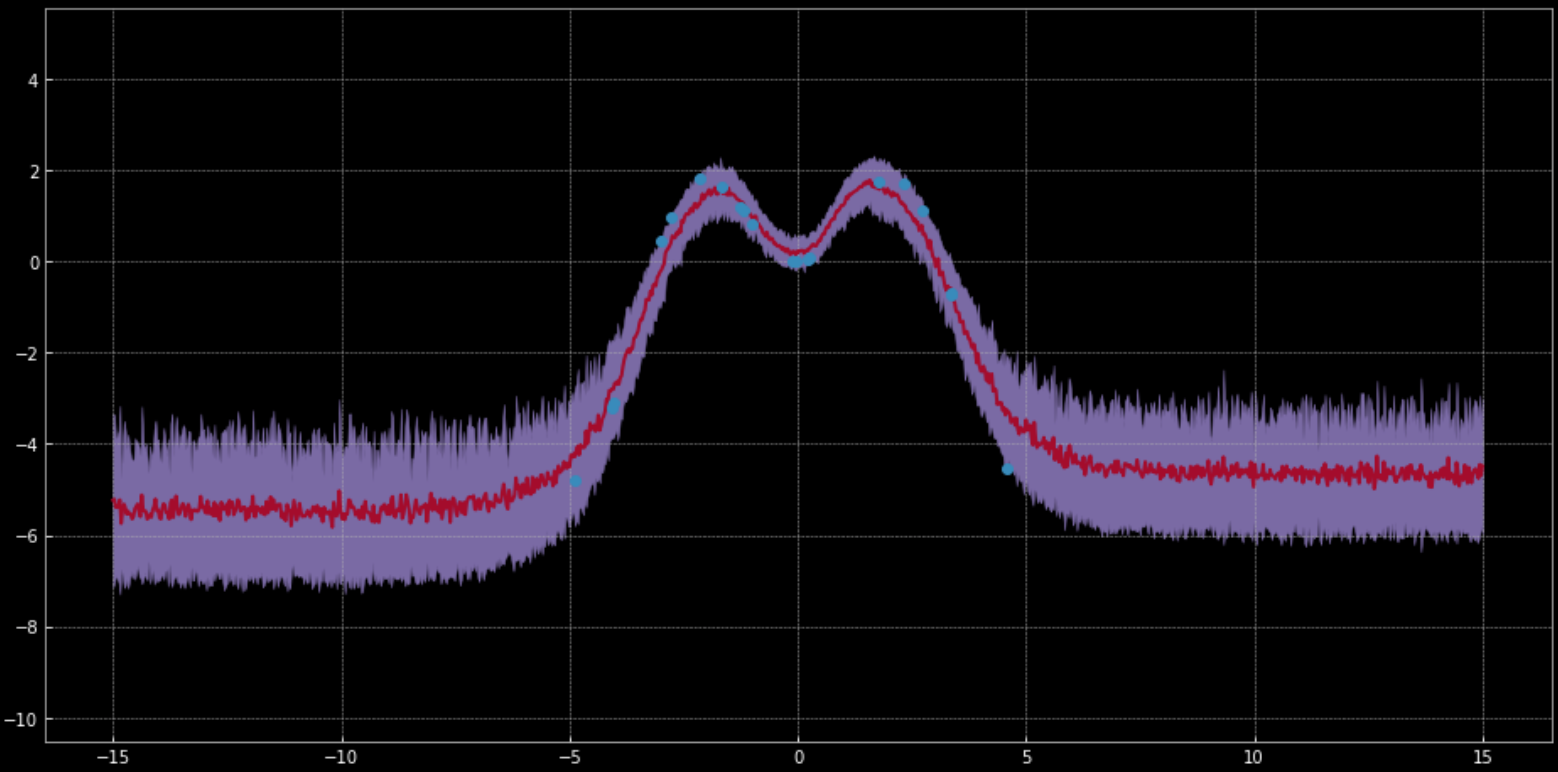
\includegraphics[width=\textwidth]{figs/exp_3.png}
    \caption{Fit Bayesian neural network (with Tanh non-linearity)}
    \label{fig:fit_BayesianNN}
\end{figure}

Fig. \ref{fig:fit_BayesianNN} provides so much more information compared to the results in Fig. \ref{fig:fit_standardNN}. The red curve shows an average of 100 evaluations, and the purple curve is mean plus/minus one standard deviation over the predictions. Thus, this plot not only presents mean estimates but also shows variances that provide uncertainty of the results. 

\begin{figure}[H]
    \centering
    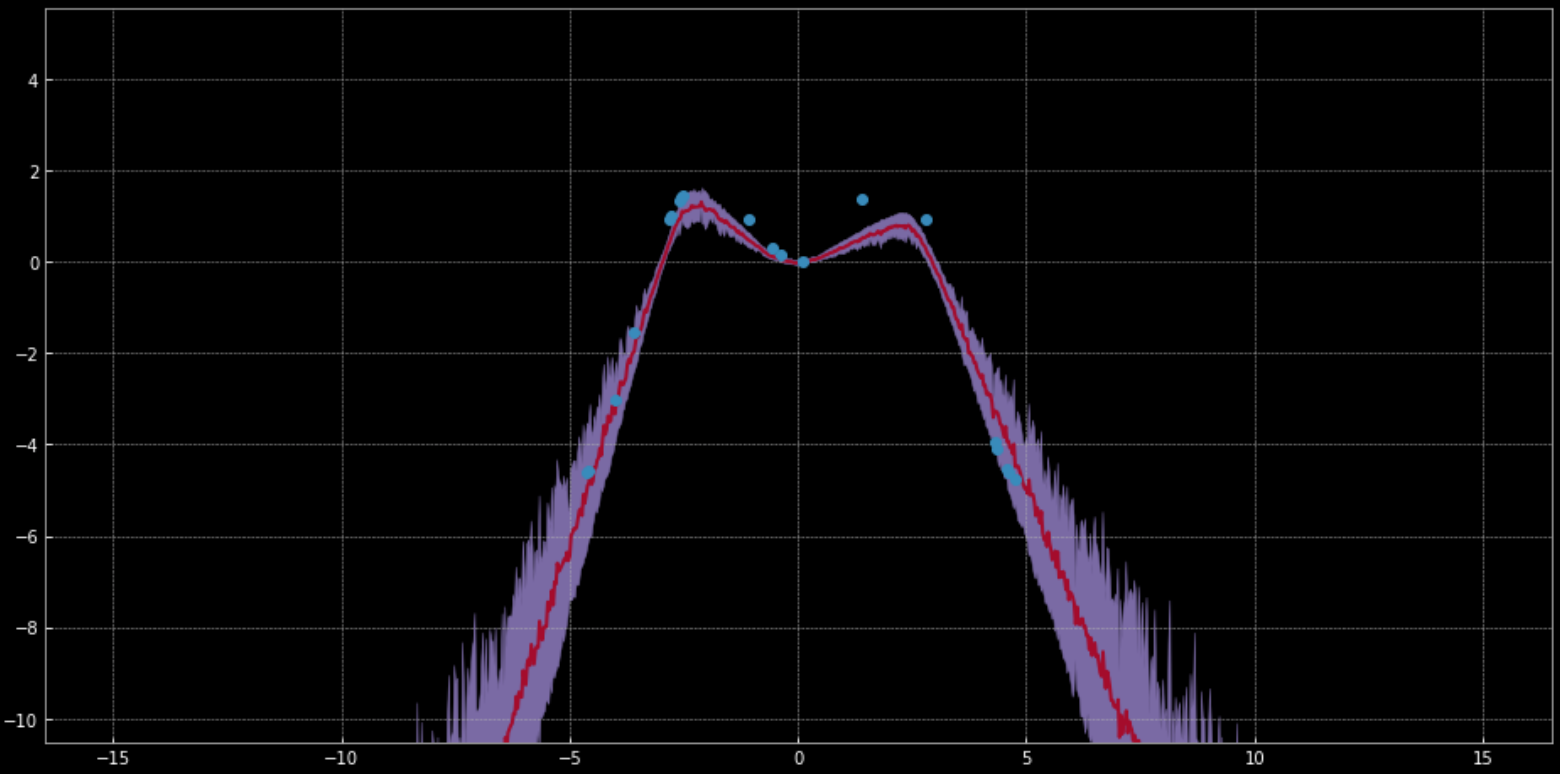
\includegraphics[width=\textwidth]{figs/exp_4.png}
    \caption{Fit Bayesian neural network (with ReLU non-linearity)}
    \label{fig:fit_BayesianNN_ReLU}
\end{figure}

Fig. \ref{fig:fit_BayesianNN_ReLU} presents estimate results using ReLU function. We note that if we use different non-linearities in our network, it provides different uncertainty estimates. It is similar to changing kernels in Gaussian process. Furthermore, the uncertainty (or variance) increases as we go farther from the training points. 
